\documentclass[a0paper,portrait]{baposter}




\usepackage{wrapfig}
\usepackage{capt-of}
\usepackage{lmodern}
\usepackage[utf8]{inputenc} %unicode support
\usepackage[T1]{fontenc}
\usepackage[colorlinks]{hyperref}


\selectcolormodel{cmyk}

\graphicspath{{figures/}} % Directory in which figures are stored


\newcommand{\compresslist}{%
\setlength{\itemsep}{0pt}%
\setlength{\parskip}{1pt}%
\setlength{\parsep}{0pt}%
}

\newenvironment{boenumerate}
  {\begin{enumerate}\renewcommand\labelenumi{\textbf\theenumi.}}
  {\end{enumerate}}



\begin{document}


\definecolor{darkgreen}{cmyk}{0.8,0,0.8,0.45}
\definecolor{lightgreen}{cmyk}{0.8,0,0.8,0.25}

\begin{poster}
{
grid=false,
headerborder=open, % Adds a border around the header of content boxes
colspacing=1em, % Column spacing
bgColorOne=white, % Background color for the gradient on the left side of the poster
bgColorTwo=white, % Background color for the gradient on the right side of the poster
borderColor=black, % Border color
headerColorOne=red, % Background color for the header in the content boxes (left side)
headerColorTwo=red, % Background color for the header in the content boxes (right side)
headerFontColor=white, % Text color for the header text in the content boxes
boxColorOne=white, % Background color of the content boxes
textborder=rounded, %rectangle, % Format of the border around content boxes, can be: none, bars, coils, triangles, rectangle, rounded, roundedsmall, roundedright or faded
eyecatcher=false, % Set to false for ignoring the left logo in the title and move the title left
headerheight=0.11\textheight, % Height of the header
headershape=rounded, % Specify the rounded corner in the content box headers, can be: rectangle, small-rounded, roundedright, roundedleft or rounded
headershade=plain,
headerfont=\Large\textsf, % Large, bold and sans serif font in the headers of content boxes
%textfont={\setlength{\parindent}{1.5em}}, % Uncomment for paragraph indentation
linewidth=2pt % Width of the border lines around content boxes
}
{}
%
%----------------------------------------------------------------------------------------
%	TITLE AND AUTHOR NAME
%----------------------------------------------------------------------------------------
%
{
\textsf %Sans Serif
{A computational study of sequential deposition: A dynamic monte carlo process in statistical physics.
}
} % Poster title
% {\vspace{1em} Marta Stepniewska, Pawel Siedlecki\\ % Author names
% {\small \vspace{0.7em} Department of Bioinformatics, Institute of Biochemistry and Biophysics, PAS, Warsaw, Pawinskiego 5a}} % Author email addresses
{\sf\vspace{0.3em}\\
Indranil Ghosh* and Budhaditya Banerjee
\vspace{0.1em}\\
\small{Department of Physics, Jadavpur University, Kolkata - 700032
}
}
{
\includegraphics{logo}} % University/lab logo


\headerbox{1. Abstract}{name=introduction,column=0,row=0, span=3}{
Few of the many enthralling applications of dynamic monte carlo process is the study of crystallization of hard spheres due to increase in pressure or the response of Ising model due to an external magnetic field switched on at an initial time, where physical time plays an integral role. In our presentation, we study a phenomenon where particles (discs) are randomly attached to a 2-dimensional surface and stay attached only if they find a required free space. With time, the number of particles that get repelled by other particles, due to not enough free spacing, increases and takes longer time to fill up the surface. We study two algorithms, a naive and then a faster-than-clock algorithm, to simulate this phenomenon of particle saturation, and compare their performances in details. We carry out the simulation with Pygame, a python package. We also calculate the approximate value of the maximum coverage numerically, for these circular particles for different radii after the simulation is carried out for a certain recommended time, with our computer programs. At last we end by investigating how Pygame can be used to carry out simulations of various monte carlo methods in algorithmic statistical physics.
}


\headerbox{2. Dynamical Monte Carlo}{name=model,column=0,below=introduction,span=1}{
Numerical studies corresponding to finding out the equilibrium close to the phase transion in Ising Model with the help of Monte Carlo methods can be \textit{a\ priori} difficult, as the equilibrium configuration is never reached during simulation. So, Dynamical Monte Carlo Method is used where the system evolves with time from one local relaxation point to another. One is mostly focused on the numerical study of the balanced configuration from a given initial configuration. In Equilibrium Monte Carlo, we have unbounded choice of configurartions manifested by the \textit{a\ priori} probability, whereas in the Dynamic Monte Carlo simulations the \textit{a\ priori} probability is fixed, which provides them with more delicacy and simplicity.

%\begin{center}
%    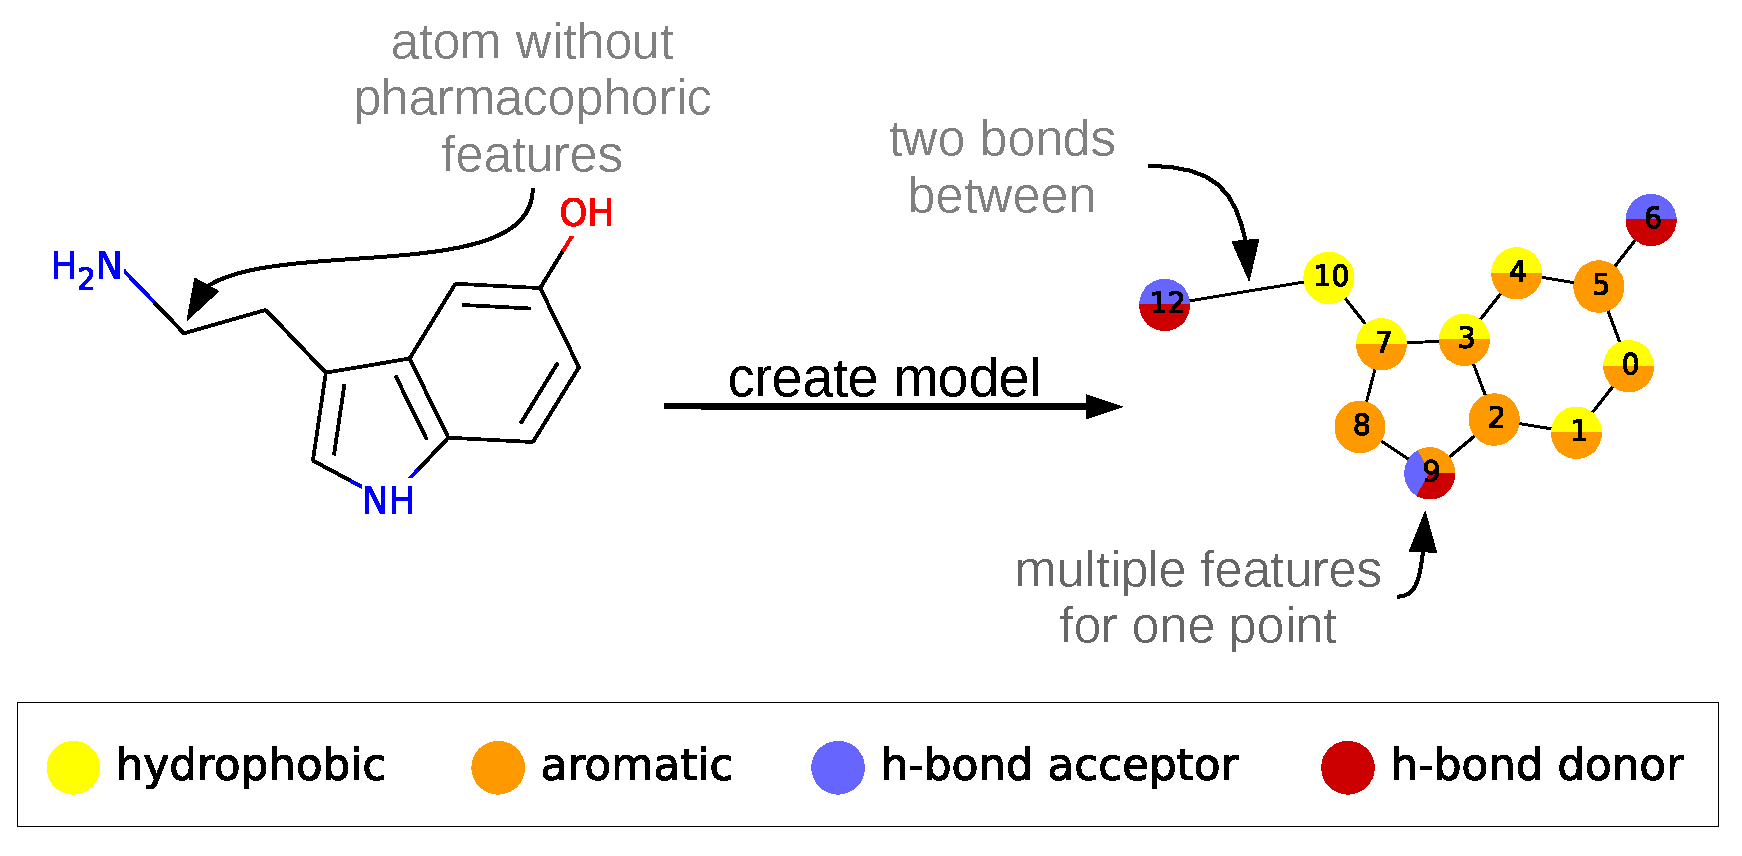
\includegraphics[width=\linewidth]{phar}
%\end{center}
%%\vspace{-2pt}
}


\headerbox{3. Naive Random Deposition}{name=mcs,column=0,below=model,span=1}{
On a 2D surface (initially a square), spherical disks are dropped randomly one after the aonther. This simulation and its analysis is congruent to the irreversible adsorption of spherical particles. Disks remain stuck to their positions where they have been deposited until and unless an overlap ocurs in which case they are removed, keeping the system unchanged. This has been implemented in Pygame that gives the position of each disks, stopping time of each sample and also calculates the maximum coverage as in \cite{zhang2013precise}. Once, enough disks have been deposited, the deposition time increases exponentially for the successive disks, in this random process, which has no memory of rejection coordinates.
%\begin{center}
%    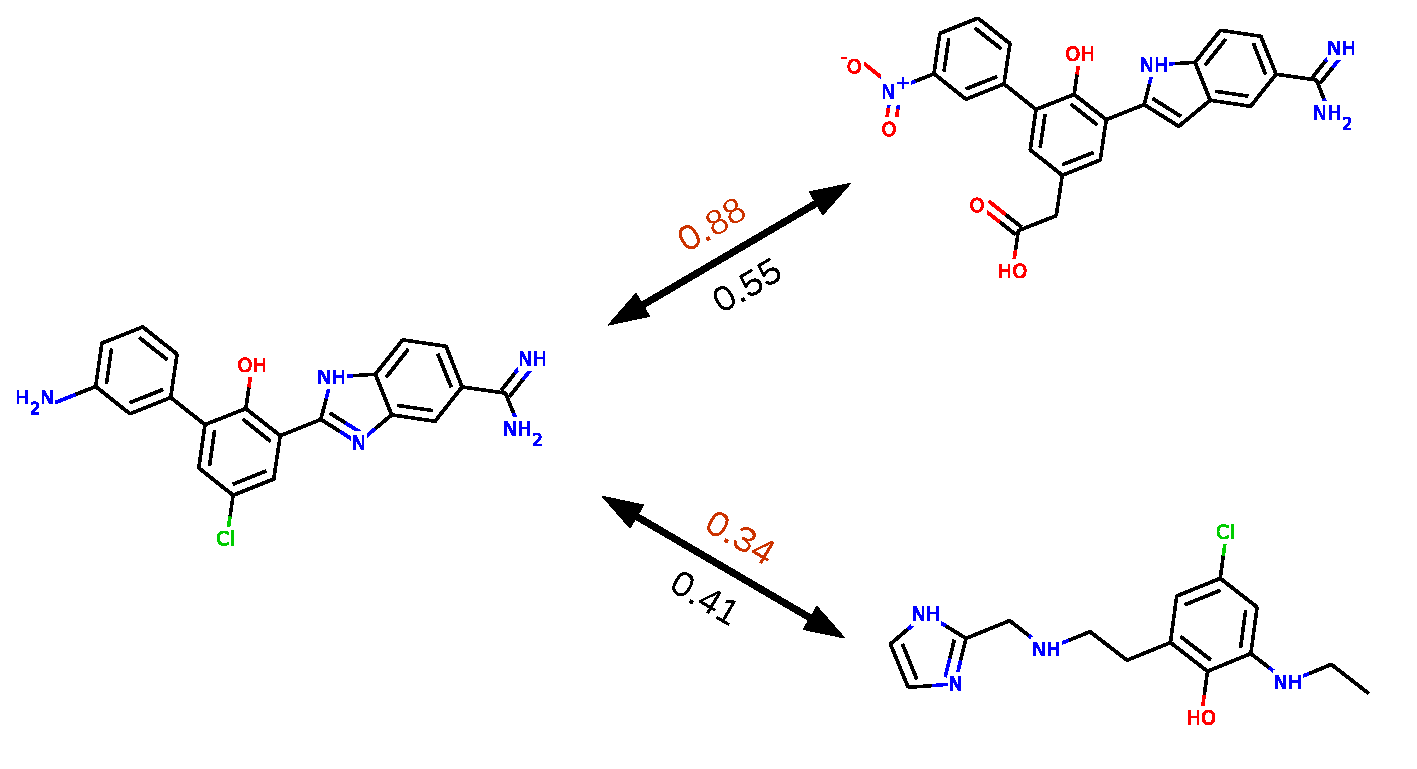
\includegraphics[width=\linewidth]{sim}
%\end{center}
}

\headerbox{4. Results}{name=screen,span=2,column=1,below=introduction}{ % To reduce this block to 1 column width, remove 'span=2'

\begin{wrapfigure}{l}{0.3\textwidth}
    \vspace{10pt}
    \begin{center}
        \includegraphics[width=\linewidth]{deposition}
    \end{center}
    \captionof{figure}{Simulation Snapshot}
    %\vspace{-145pt}
\end{wrapfigure}

The coverage values calculated numerically for different radii are as follows: 
\begin{itemize}
\item 0.04: 0.5127079210658543
\item 0.06: 0.49762827632862316
\item 0.08: 0.4423362456254428
\end{itemize}

\vspace{-5pt}
\begin{center}
    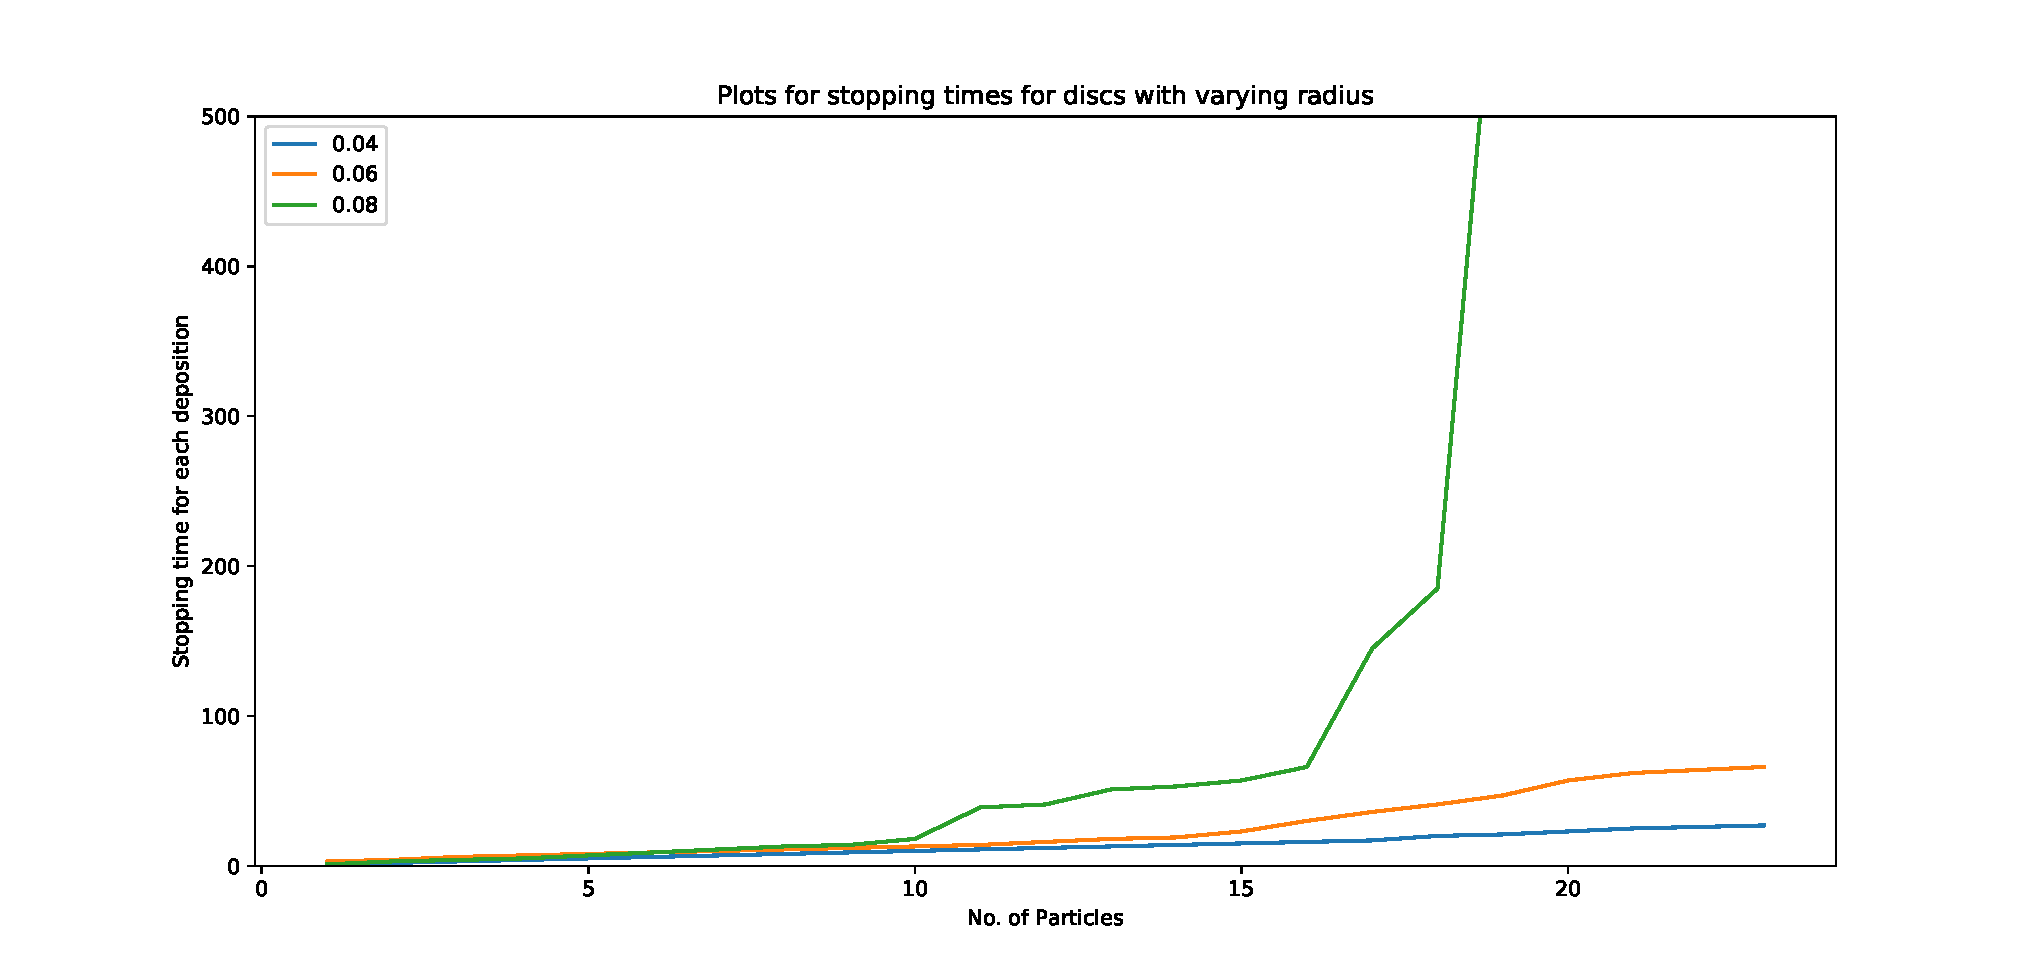
\includegraphics[width=0.85\linewidth]{plot}
\end{center}
\captionof{figure}{Deposition Stopping Time Plot}
}


\headerbox{5. Faster Than The Clock Algorithm}{name=sea,span=2,column=1,below=screen}{ % To reduce this block to 1 column width, remove 'span=2'

%\begin{wrapfigure}{l}{0.3\textwidth}
%    \vspace{10pt}
%    \begin{center}
%        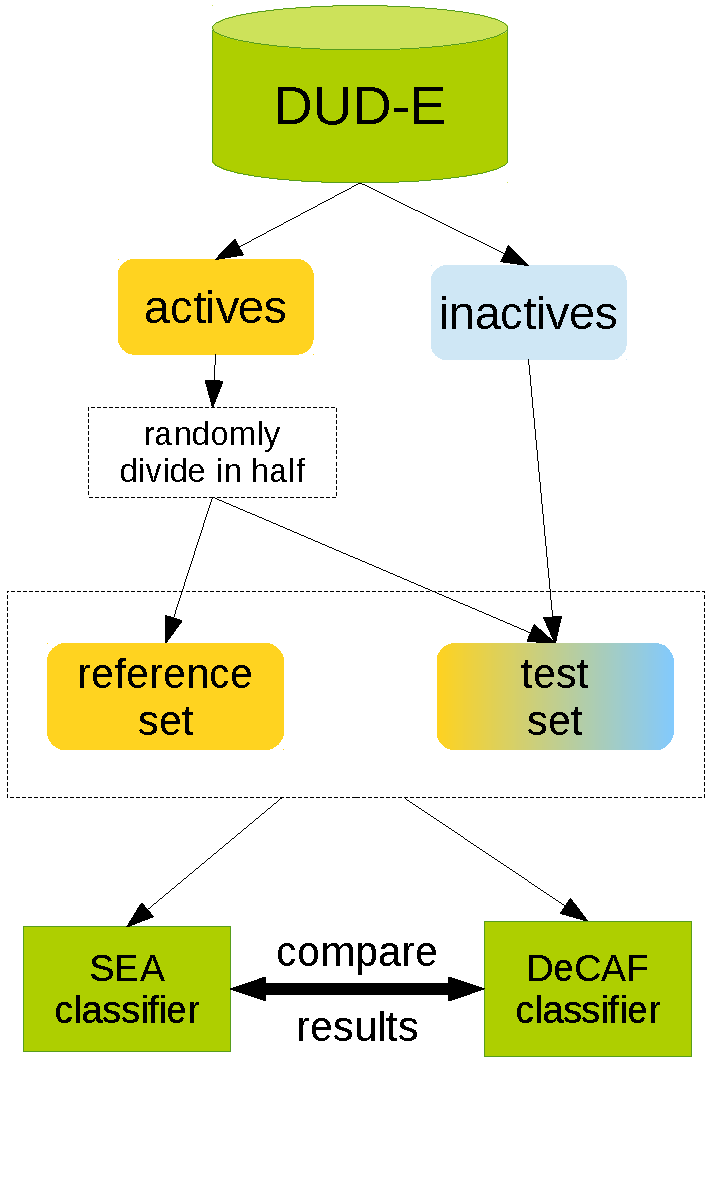
\includegraphics[width=\linewidth]{class}
%    \end{center}
%    %\vspace{-145pt}
%\end{wrapfigure}

% We tested DeCAF in 35 case studies taken from the DUD-E database, to evaluate its power to discriminate between active and inactive molecules.
% We used DeCAF as a classifier and compared it to the SEA (Similarity Ensemble Approach) algorithm \cite{keiser2007relating}.
% To compare sets of ligands, we adapted the approach used in SEA, replacing Tc by DCAF.
% We prepared datasets as shown in the left diagram.
% Then, we tested both classifiers calculating ROC AUC values for every target (below).
As Werner Krauth \cite{krauth2006statistical} mentions, the DMC methods focus on the accessible regions in the simulation, where new particles can be deposited successfully. After a large number of depositions, $\Delta_t$ until the next successful deposition is a random variable. If $\lambda$ is the probability of deposit rejection, then \begin{equation}
\lambda = 1 - \frac{area\ of\ accessible\ region}{area\ of\ deposition\ region},\ \\
\Delta_t = 1 + int[\frac{log\ ran(0,1)}{log\ \lambda}]
\end{equation} 
The total area of accessible region is computed by cutting it up into smaller regions $\{R_1, R_2, ..., R_k\}$, such that these small regions do not contain any holes. The vectors $\{(x_1, y_1), (x_2, y_2), ..., (x_n, y_n)\}$ form the vertices of a polygon that spans the small region $R_k$. The polygon has the area:\begin{equation}
A = \frac{x_1y_2 + ... + x_ny_1}{2} - \frac{x_2y_1 + ... + x_1y_n}{2}
\end{equation}
The circular segments must then be subtracted to get the accessible region from $R_k$. The sum of all these areas gives the total accessible area which lets us calculate $\lambda$ and $\Delta_t$. A disk can now be placed successfully on the accessible space. The probability of a disk falling on a region $R_k$ can be computed using Tower Sampling. The process is iteratively carried out unitil a disk is placed successfully. This algorithm advocating geometric computations is much faster than the naive approach. All the codes are available at {\color{red} https://github.com/indrag49/Computational-Stat-Mech} and can be easily implemented with Pygame.
% Please ask me about details.

%\hspace{0pt}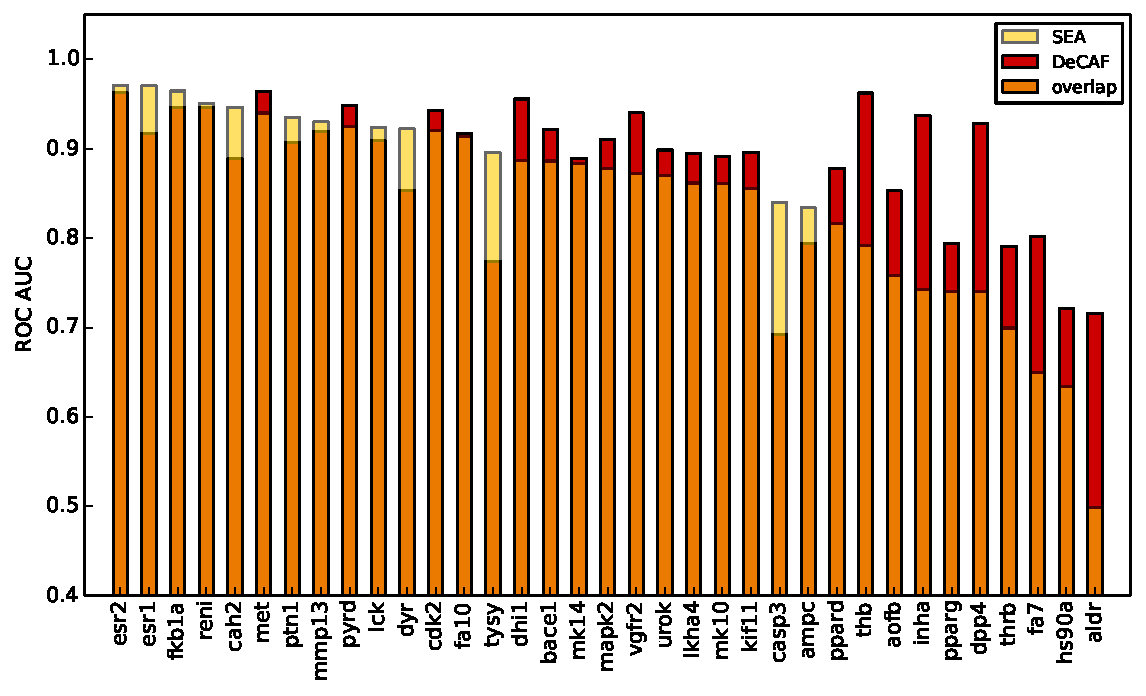
\includegraphics[width=0.95\linewidth]{res}

}


\headerbox{6. Pygame in Simulating Statistical Physics}{name=conclusion,column=1,below=sea,span=2,above=bottom}{
% DeCAF is a chemoinformatical tool that can be helpful in ligand-based drug design.
% It provides a comprehensive molecule description and a fast algorithms for comparing and aligning multiple ligands.
Pygame\cite{sweigart2012making} framework provides additional modularities for drawing graphics, playing sounds, handling mouse input, etc. i.e., creating programs with a Graphical User Interface. Many of the computational Statistical Mechanics simulations were run with the Pygame:
\begin{boenumerate}\compresslist
    \item Perfect Sampling with Markov Chains was demonstrated with the simulation of the $3X3$ pebble game.
    \item Event driven Molecular Dynamics simulation of the hard spheres manifesting their collisions were also carried out.
    \item Simulation of sampling a path contributing to free density function, using L\'evy construction was also brought about.
\end{boenumerate}
% It can be also used in other [procedures], such as database screening or drug repositioning.
% DeCAF is written in Python and freely available at \textbf{\color{darkgreen}http://bitbucket.org/marta-sd/decaf}. 
}


\headerbox{7. References}{name=references,column=0,span=1,below=mcs,above=bottom}{


%\small % Reduce the font size in this block
\renewcommand{\section}[2]{\vskip 0.05em} % Get rid of the default "References" section title
%\nocite{*} % Insert publications even if they are not cited in the poster


\bibliographystyle{unsrt}
\bibliography{poster} % Use sample.bib as the bibliography file
}

\end{poster}

\end{document}
